\documentclass[12pt]{scrartcl}

 

\usepackage[utf8]{inputenc}

\usepackage[T1]{fontenc}

\usepackage{lmodern}

\usepackage[ngerman]{babel}

\usepackage{amsmath}

\usepackage{graphicx}


 

\title{Versuch E1\\ Drehspulinstrument}

\author{Frederik Strothmann, Henrik Jürgens}

\date{\today}


\begin{document}


 %deckblatt erstellen

\maketitle
\tableofcontents
\newpage


%einleitung zu dem experiment

\section{Einleitung}

Ein einfaches Drehspulinstrument soll durch Wahl geeigneter Vor- und Parallelwiderstände
zur Messung von Strömen und Spannungen verwendet werden.
Die Elektromotorische Kraft (EMK) und der Innenwiderstand sind wichtige Kenngrößen einer Spannungsquelle.

Im Rahmen dieses Versuchs sollen diese beiden Größen einer Batterie ausgemessen werden.
Nichtlineare Widerstandselemente spielen eine wichtige Rolle auf dem Gebiet der Elek-
tronik. Ausgemessen werden soll die Strom–Spannungs–Charakteristik einer Glühlampe
und einer Halbleiterdiode.
%versuchsaufbau mit skizze

\section{Versuchsaufbau}
Der Versuchaufbau besteht aus einem Netzgerät, digitalen- und analogen Multimeter, sowie ein Versuchkasten, welcher mit fünf Wiederstängen, einer Diode, einer Lampe, einer Batterie und einem Drehspulinstument versehen ist. Die Komponenten haben alle vorgefertigte Kontakte zum verbinden.


\begin{figure}[htbp] 
  \centering
    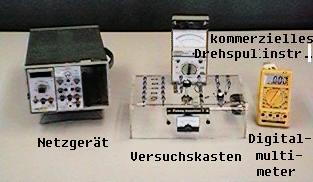
\includegraphics[scale = 0.5]{versuchsaufbau.JPG}
  	\caption[Foto der für den Versuch verwendeten Geräte]{Foto der für den Versuch verwendeten Geräte\footnotemark}
  \label{fig:versuchsaufbau}
\end{figure}
\footnotetext{Graphik wurde am 13.08.2014 von der Seite: http://www.atlas.uni-wuppertal.de/~kind/apjpg/ap1e1a.JPG entnommen}

Die Aufbauten der Aufgaben werden bei der jeweiligen Durchführung angegeben.

\section{Versuchsdurchführung}


\subsection{Praktische Durchführung}

\begin{enumerate}

	\item 
	Berechnen Sie den Innenwiderstand 				eines Drehspulmeßgerätes. Das Instrument
	zeigt Vollausschlag bei einem Strom von 			1 mA bzw. einer Spannung von 200 mV.
	\item
	Bauen Sie aus diesem Instrument mit 				Hilfe der Ihnen zur Verfügung stehenden 			Widerstände $\text{R}_1$ bis 					$\text{R}_5$ ein 								Strommeßgerät mit Vollausschlag bei 300 			mA. Wie groß ist sein Innenwiderstand?
	\item
	Das soeben gebaute Strom-Meßinstrument 			soll bei der Bestimmung des unbekannten 			Widerstands $\text{R}_x$ benutzt werden. 	Der Widerstand soll durch Strom- und 			Spannungsmessung mit Hilfe von zwei 				Schaltungen bestimmt werden.
	
	\begin{figure}[htbp] 
	  \centering
	    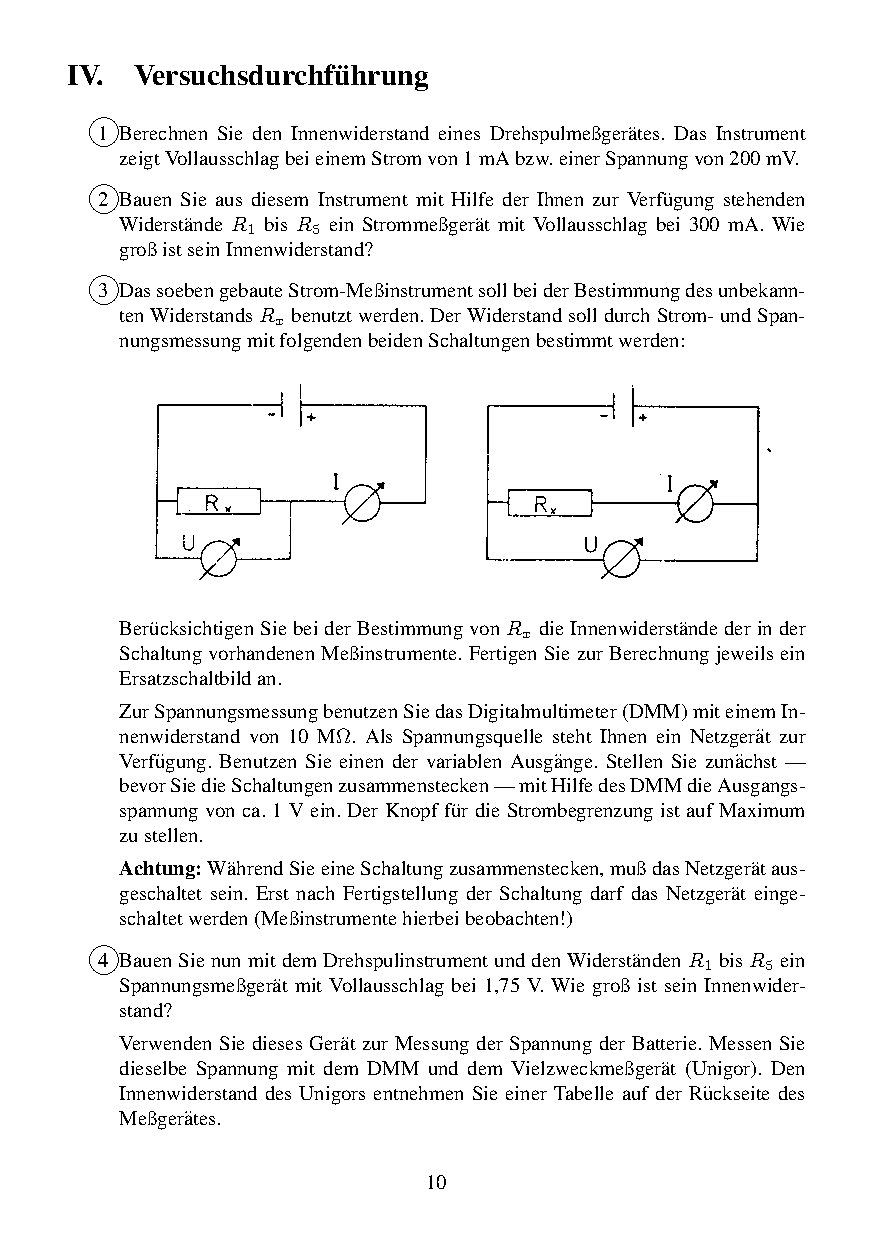
\includegraphics[trim = 20mm 107mm 20mm 60mm, clip, scale = 1]{abb_versuch_3.pdf}
	  	\caption[Abbildung der beiden Schaltungen, für die Bestimmung des Wiederstandes]{Abbildung der beiden Schaltungen, für die Bestimmung des Wiederstandes\footnotemark}
	  \label{fig:abb_versuch_3}
	\end{figure}
	\footnotetext{Abbildung entnommen von http://www.atlas.uni-wuppertal.de/~kind/E1.pdf Seite 10 am 16.08.2014}
	
	Berücksichtigen Sie bei 	der Bestimmung 			von $\text{R}_x$ die Innenwiderstände 			der in der Schaltung vorhandenen 				Meßinstrumente. Fertigen Sie zur 				Berechnung jeweils ein Ersatzschaltbild 			an. Zur Spannungsmessung benutzen Sie 			das Digitalmultimeter (DMM) mit einem 			Innenwiderstand von 10 M$\Omega$. Als 			Spannungsquelle steht Ihnen ein 					Netzgerät zur Verfügung. Benutzen Sie 			einen der variablen Ausgänge. Stellen 			Sie zunächst -- bevor Sie die 					Schaltungen 	zusammenstecken -- mit Hilfe 	des DMM die Ausgangsspannung von ca. 			1 V ein. Der Knopf für die 						Strombegrenzung ist auf Maximum zu 				stellen.
	\item
	Bauen Sie nun mit dem Drehspulinstrument 	und den Widerständen $\text{R}_1$ bis 			$\text{R}_5$ ein Spannungsmeßgerät mit 			Vollausschlag bei 1,75 V. Wie groß ist 			sein Innenwiderstand? Verwenden Sie 				dieses Gerät zur Messung der Spannung 			der Batterie. Messen Sie dieselbe 				Spannung mit dem DMM und dem 					Vielzweckmeßgerät (Unigor). Den 					Innenwiderstand des Unigors entnehmen 			Sie einer Tabelle auf der Rückseite des 			Meßgerätes. Erklären Sie die 					unterschiedlichen Meßergebnisse.
	(Die Batterie sollte nur durch 					kurzen Druck auf den Taster belastet 			werden. Warum?)
	\item
	Messen Sie den Innenwiderstand der 				Batterie. Er wird größer sein als bei 			einer normalen Batterie, da ein 					”zusätzlicher Innenwiderstand“ eingebaut 	ist. Verwenden Sie zur Spannungsmessung 			das Vielzweckinstrument (Unigor). Messen 	Sie U und I und tragen Sie U gegen I 			auf. Bestimmen Sie $\text{U}_0$ und 				$\text{R}_i$.
	
	\begin{figure}[htbp] 
	  \centering
	    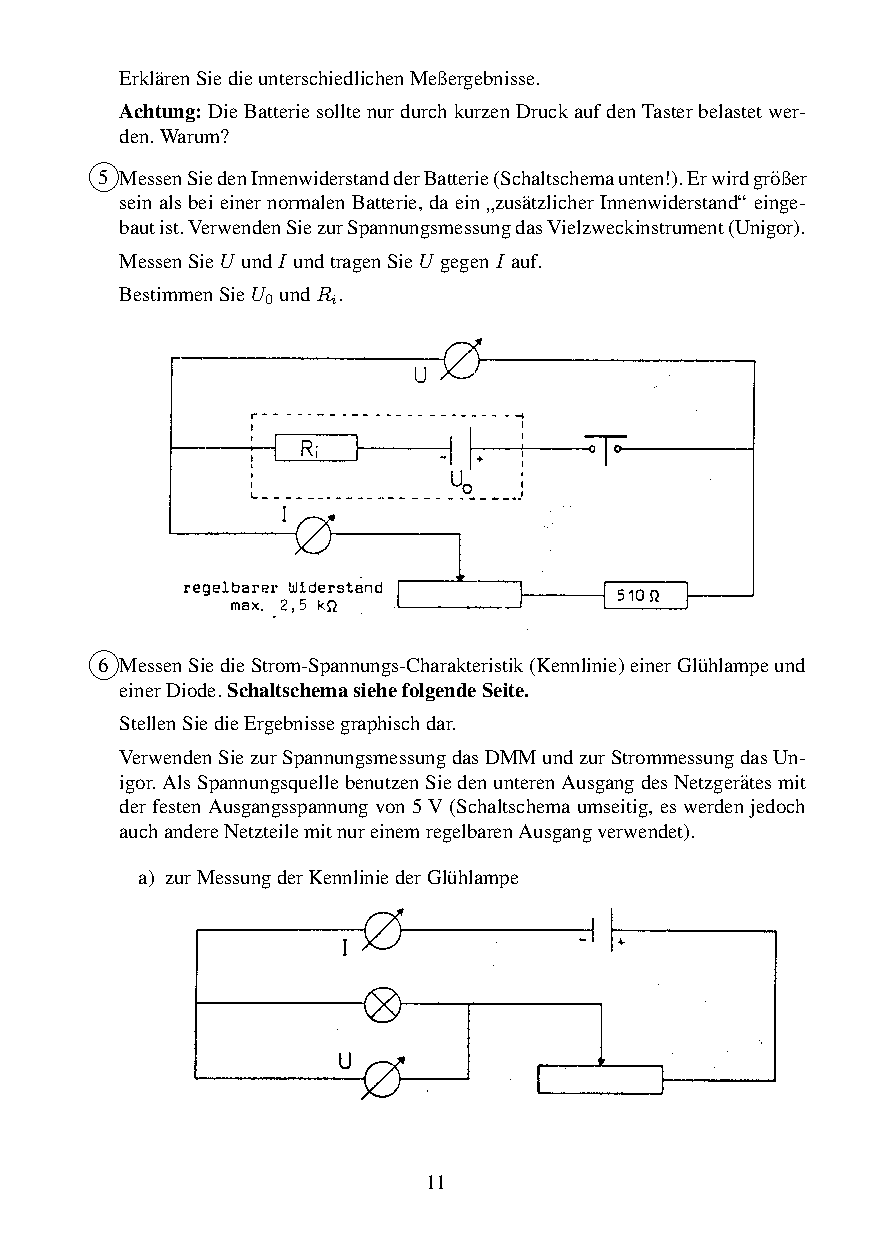
\includegraphics[trim = 1mm 102mm 1mm 55mm, clip, scale = 1]{abb_versuch_5_6a.pdf}
	  	\caption[Abbildung der Schaltung, für die Bestimmung des Wiederstandes R und der Spannung U]{Abbildung der Schaltung, für die Bestimmung des Wiederstandes R\textsubscript{i} und der Spannung U\textsubscript{0}\footnotemark}
	  \label{fig:abb_versuch_5}
	\end{figure}
	\footnotetext{Abbildung entnommen von http://www.atlas.uni-wuppertal.de/~kind/E1.pdf Seite 11 am 16.08.2014}
	\newpage
	
	\item
	Messen Sie die Strom-Spannungs-					Charakteristik (Kennlinie) einer 				Glühlampe und einer Diode. Stellen Sie 			die Ergebnisse graphisch dar. Verwenden 			Sie zur Spannungsmessung das DMM und zur 	Strommessung das Unigor. Als 					Spannungsquelle benutzen Sie den unteren 	Ausgang des Netzgerätes mit einer 				Ausgangsspannung von 5 V.
	
	a) zur Messung der Kennlinie der 				Glühlampe
	
	\begin{figure}[htbp] 
	  \centering
	    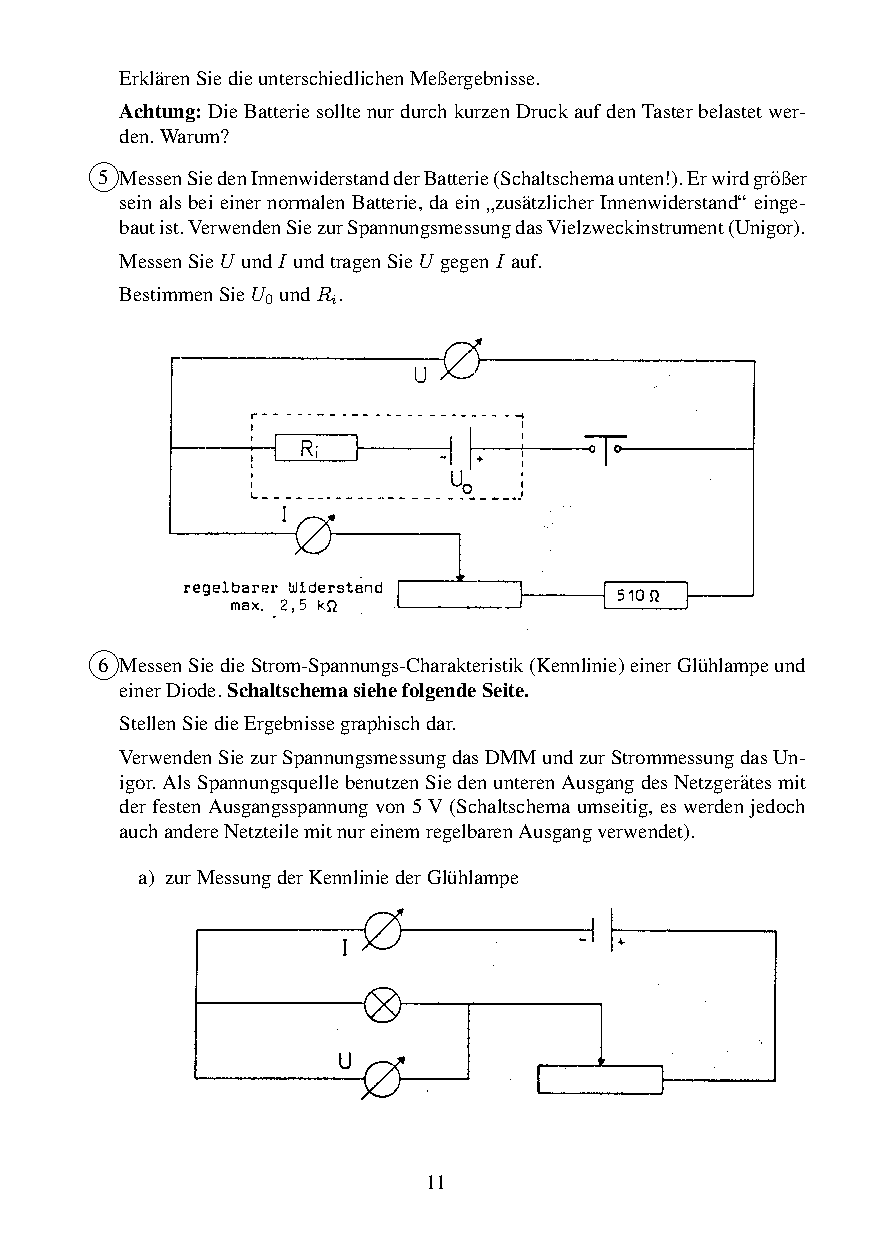
\includegraphics[trim = 18mm 15mm 1mm 151mm, clip, scale = 1]{abb_versuch_5_6a.pdf}
	  	\caption[Abbildung der Schaltung, für die Bestimmung der Kennlinie der Glühlampe]{Abbildung der Schaltung, für die Bestimmung der Kennlinie der Glühlampe\footnotemark}
	  \label{fig:abb_versuch_6a}
	\end{figure}
	\footnotetext{Abbildung entnommen von http://www.atlas.uni-wuppertal.de/~kind/E1.pdf Seite 11 am 16.08.2014}
	\newpage
	b) zur Messung der Kennlinie einer Diode
	
	\begin{figure}[htbp] 
 	 \centering
 	   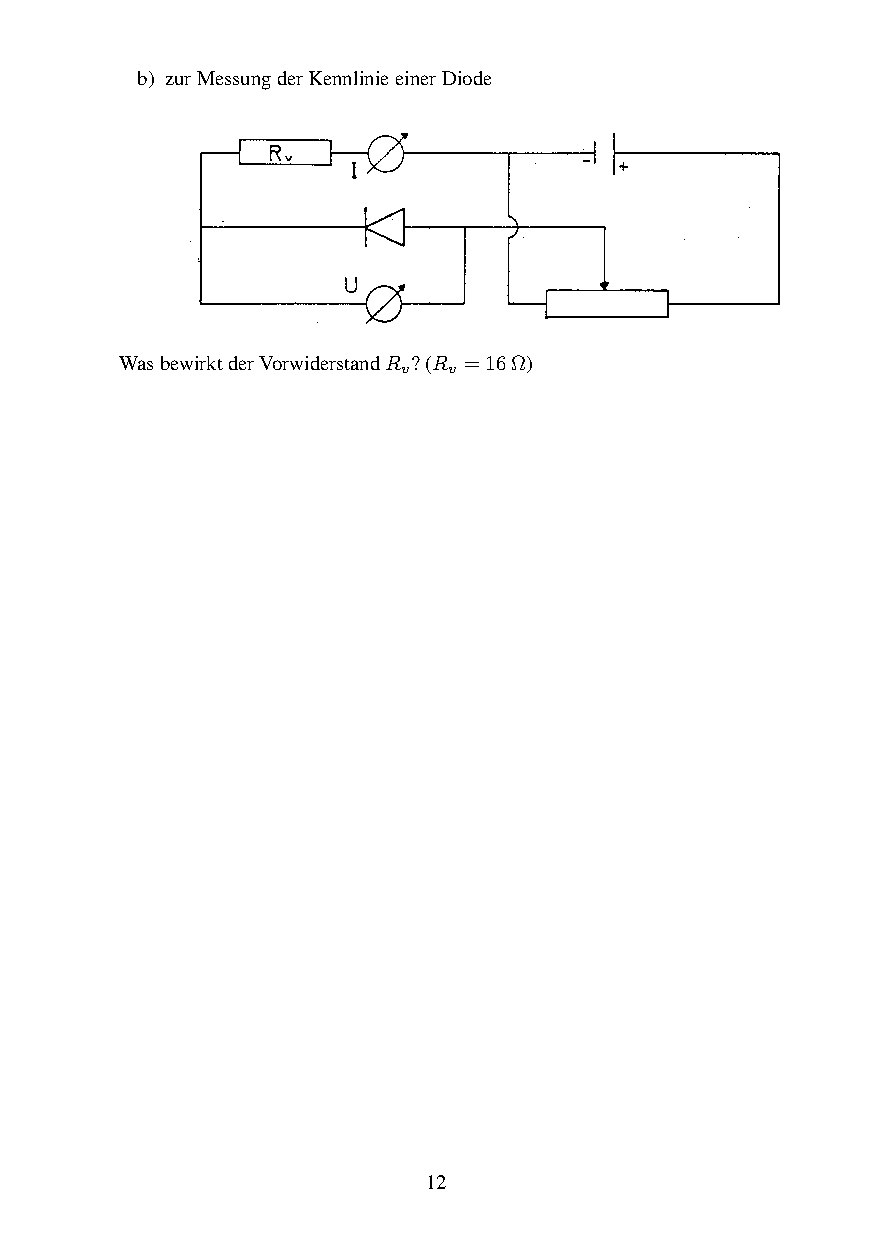
\includegraphics[trim = 1mm 152mm 1mm 15mm, clip, scale = 1]{abb_versuch_6b.pdf}
  	\caption[Abbildung der Schaltung, für die Bestimmung der Kennlinie der Diode]{Abbildung der Schaltung, für die Bestimmung der Kennlinie der Diode\footnotemark}
  	\label{fig:abb_versuch_6b}
	\end{figure}
	\footnotetext{Abbildung entnommen von http://www.atlas.uni-wuppertal.de/~kind/E1.pdf Seite 12 am 16.08.2014}
	Was bewirkt der Vorwiderstand
	$\text{R}_v? (\text{R}_v= 16\Omega)$
\end{enumerate}


\subsection{Theoretische Durchführung}

\begin{enumerate}

	\item
	Um den Innenwiderstand R$_i$ des 				Drehspulmeßgerätes zu bestimmen benutzen 	wir die Formel:
	\begin{align}
	\text{R}_{i}= \frac{\text{U}_0}					{\text{I}_k}
	\end{align}
	U$_0$ die EMK, I$_k$ der Klemmenstrom.
	
	Fehler:
	\begin{align}
	\sigma_{\text{R}_i} = 							\sqrt{\left(\frac{1}{\text{I}_k}\sigma_{\text{U}_0}\right)^2
	+\left(\frac{\text{U}_0}{(\text{I}_k)^2}\sigma_{\text{I}_k}\right)^2}
	\end{align}	 
	\item
	%Gesamtwiderstand muss ausgerechnet werden
	\item
	Die beiden Formeln für den Widerstand 			R$_x$ sind:
	\begin{align}
	\text{R}_x=\frac{\text{U}}						{\text{I}}-\text{R}_{i_I}
	\end{align}
	\begin{align}
	\text{R}_x= 										\frac{\text{U}\text{R}_{i_U}}					{\text{I}\text{R}_{i_U}-\text{U}}
	\end{align}
	U die am Digitalmultimeter gemessene 			Spannung, I der am Drehspulinstrument 			gemessene Strom, R$_{i_I}$ der 					Innenwiderstand des Drehspulinstruments 			und R$_{i_U}$ die am Digitalmultimeter 			gemessene Spannung.
	
	Fehler:
	\begin{align}
	\sigma_{\text{R}_x}=
	\sqrt{\left(\frac{1}								{\text{I}}\sigma_U\right)^2+
	\left(\frac{U}{I^2}\sigma_I\right)^2+
	\left(\sigma_{\text{R}_{i_I}}\right)^2}
	\end{align}		
	\begin{align}
	\sigma_{\text{R}_x}=
	\sqrt{\left(\frac{\text{I}
	\text{R}_{i_U}^2}								{(\text{I}\text{R}_{i_U}-
	\text{U})^2}\sigma_U\right)^2+
	\left(\frac{\text{U}\text{R}_{i_U}^2}			{(\text{I}\text{R}_{i_U}-
	\text{U})^2}\sigma_I\right)^2+
	\left(\frac{\text{U}}							{(\text{I}\text{R}_{i_U}-
	\text{U})^2}\sigma_{
	\text{R}_{i_U}}\right)^2}
	\end{align}	 
	\item
	%Während des Versuchs Dokumentieren
	\item
	\item
	
\end{enumerate}


\section{Messergebnisse}



\section{Auswertung}


\section{Diskussion}


 %Werte stimmen mit den Formeln überein/nicht überein

\end{document}

